\chapter{Validazione}

In questo capitolo viene validato il lavoro svolto e vengono presentati i risultati ottenuti.
% test della libreria sviluppata sono stati effettuati su reti locali di diverse dimensioni, struttura e ,soprattutto, diversi dispositivi.
%Le reti analizzate per la validazione della libreria 
La validazione della libreria sviluppata \'e stata effettuata su effettive reti locali che differiscono tra di loro per struttura di rete, numero e tipo di dispositivi.
Questa scelta ha quindi reso possibile la verifica della bont\`a delle euristiche proposte su una quantit\`a ed un tipo di traffico molto disparati.
In aggiunta, la conoscenza della topologia della rete, ha permesso di comparare i risultati ottenuti mediante l'utilizzo della libreria con la struttura effettiva della rete.

I risultati ottenuti verranno presentati grafi realizzati usando Graphviz\cite{graphviz} in cui vengono evidenziate le topologie delle reti prese in analisi.
Durante la validazione del lavoro svolto \'e stato di fondamentale utilit\`a anche il software Wireshark \cite{wireshark}.
Questo analizzatore di pacchetti open-source ha permesso, insieme alla conoscenza delle reti su cui si sono eseguite le prove, di ispezionare ogni pacchetto alla ricerca di possibili inconsistenze con la soluzione proposta. 

Le reti su cui sono state effettuate le prove possono essere suddivise in tre categorie:
\begin{itemize}
	\item Reti semplici: topologia basilare, dispositivi connessi direttamente ad un access point.
	\item Reti con repeater: topologia di rete variabile, presenza di repeater e di dispositivi connessi ad essi.
	\item Reti complesse: topologia complessa, reti di tipo professionale.
\end{itemize}
Per motivi di privacy parte degli indirizzi MAC ed SSID verranno censurati.


%I risultati ottenuti sono stati  comparati con l'effettiva topologia della rete %convalidati dalla conoscenza della topologia della rete che si sta cercando di analizzare 
%File .pcap e prove sul campo + dot
%Wireshark
%AP e Repeater, meta' indirizzo local rep e meta' indirizzo scheda

\newpage 
\section{Analisi della topologia di rete}
\subsubsection{Reti semplici}

Il primo esempio presentato in figura \ref{fig:es1} rappresenta una cattura effettuata in una rete locale domestica in cui, al momento dell'esecuzione, erano connessi due dispositivi.
La topologia di questa rete \'e relativamente banale ed \'e costituita da due dispositivi, tra cui una smart TV in riproduzione mediatica, direttamente connessi all'access point.
%nonna.pcap

\begin{figure}[!h]
	\centering
	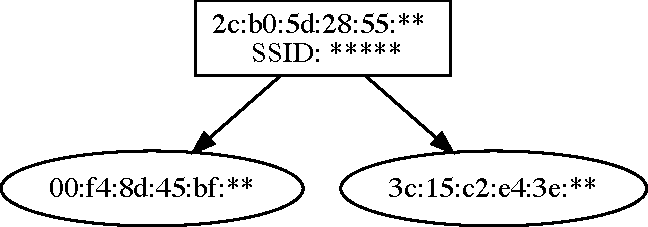
\includegraphics{images/img8censored.pdf}
	\caption{Primo esempio}
	\label{fig:es1}
\end{figure}


Nel grafo \ref{fig:es2} si mostra l'evoluzione topologica della stessa rete in un diverso momento della giornata, in questo caso si pu\`o notare la presenza di diversi nuovi dispositivi collegati.
%nonna3.pcap
\begin{figure}[!h]
	\centering
	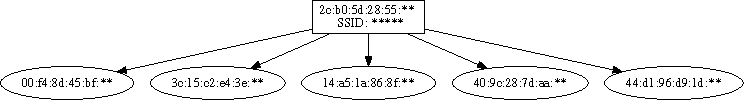
\includegraphics{images/img9censored.pdf}
	\caption{Secondo esempio}
	\label{fig:es2}
\end{figure}

La scelta di queste catture come primo esempio \'e riconducibile non solo alla semplice struttura della rete ma anche ad una semplicit\`a del traffico analizzato.
Una veloce analisi dei pacchetti catturati effettuata con il software Wireshark mostra, infatti, l'uso esclusivo di indirizzi MAC globalmente assegnati unicast e nessun tipo di repeater collegato alla rete.
Inoltre, l'access point utilizza un singolo indirizzo MAC: sia per effettuare le operazioni di annuncio di rete tramite frame beacon che per interagire con i dispositivi connessi.

Una prima validazione delle euristiche utilizate pu\`o essere invece vista nella figura \ref{fig:es3}.
Il numero di dispositivi \'e di nuovo limitato ma in questo caso, analizzando i pacchetti catturati, si pu\`o notare la presenza di diversi indirizzi MAC legati al router ed un uso di indirizzi multicast.
Il beacon frame della rete in esame viene infatti trasmesso attraverso l'uso di un indirizzo localmente assegnato, mentre le operazioni come trasmissione di frame data vengono effettuate utilizzando l'effettivo indirizzo MAC del dispositivo.
Una particolarit\`a di questa topologia \'e nell'utilizzo di indirizzi multicast dei dispositivi collegati per l'invio di frame di tipo controllo che vengono correttamente gestiti dalla libreria sviluppata.

%Fermo - Multicast

\begin{figure}[!h]
	\centering
	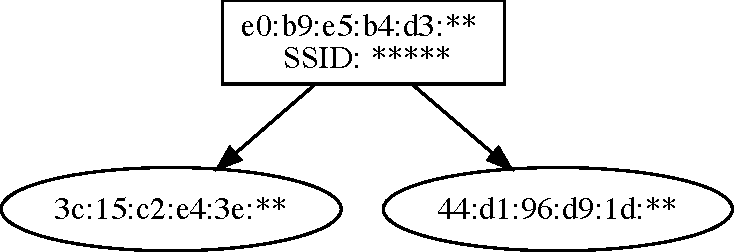
\includegraphics{images/img10censored.pdf}
	\caption{Terzo esempio}
	\label{fig:es3}
\end{figure}


L'ultima cattura presentata per questa sezione in figura \ref{fig:es4} proviene da una rete 5G i cui dispositivi connessi sono principalmente smartphone e smart speaker quali Google Home.
Data la possibilit\`a di questo router di operare simultaneamente in dual-band, annunciando quindi reti in 2G e 5G, le euristiche implementate sono fondamentali per gestire i numerosi indirizzi MAC localmente assegnati che operano nelle due diverse bande.
Questo tipo di cattura mostra anche come la soluzione proposta sia in grado di identificare dispositivi spesso inattivi, quali smart speaker, con un minimo traffico di rete. 


\begin{figure}[!h]
	\centering
	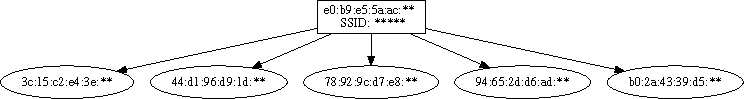
\includegraphics{images/img11censored.pdf}
	\caption{Quarto esempio}
	\label{fig:es4}
\end{figure}

%Casa

\newpage

\subsubsection{Reti con repeater}

Per la validazione su reti con topologia pi\`u complessa sono stati effettuate delle prove con diversi repeater Wi-Fi.

Il primo esempio che si riporta in figura \ref{fig:es5} riguarda l'introduzione di un repeater in una rete gi\`a presentata.
Il traffico analizzato mostra come, in questo caso, il repeater agisca in maniera "trasparente", aggiungendo il suo indirizzo MAC come trasmettitore nei frame riguardanti i dispositivi a lui connesso.
In aggiunta nella rete \'e presente un dispositivo di tipo IoT che, oltre ad interagire con i dispositivi interni, effettua annunci della propria rete locale.
%CasaRepeater

\begin{figure}[!h]
	\centering
	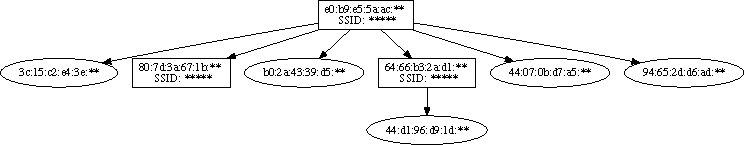
\includegraphics{images/img12censored.pdf}
	\caption{Quinto esempio}
	\label{fig:es5}
\end{figure}


Si presenta ora una delle catture pi\`u significative per la validazione della soluzione proposta.
La rete in esame in figura \ref{fig:es6} \'e composta da un router collegato tramite cavo ad un access point che fornisce connettivit\`a Wi-Fi.
A sua volta a questo viene collegato un repeater che verr\`a utilizzato dai dispositivi per usufruire della connessione.

\begin{figure}[!h]
	\centering
	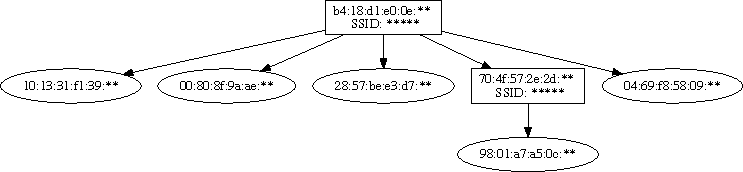
\includegraphics{images/img13censored.pdf}
	\caption{Sesto esempio}
	\label{fig:es6}
\end{figure}
%Wifi_repeater

Il repeater utilizzato in questa configurazione, pur differendo da quello presentato nel precedente esempio solo per il firmware in uso, ha un comportamento totalmente diverso.
Vengono utilizzati un numero di indirizzi MAC localmente assegnati pari al numero di dispositivi a lui collegati il cui valore \'e pari ad una composizione del LAA del repeater e del NIC del dispositivo.
Le euristiche presentate nel precedente capitolo riescono, come mostrato in figura, a classificare correttamente questo scenario.
I valori To DS e From DS presentati nel capitolo precedente permettono, inoltre, di identificare il collegamento tra router ed access point come cablato.
Infatti, dall'analisi del traffico, si pu\`o notare un cambio di mezzo trasmissivo tra access point e router ed un una mancanza di quest'ultimo di metriche Wi-Fi.

L'ultimo esempio che si riporta in figura \ref{fig:es7} riguarda un'altra rete locale con la presenza di repeater che non utilizza indirizzi localmente assegnati per la gestione dei dispositivi a lui connessi.
  
\begin{figure}[!h]
	\centering
	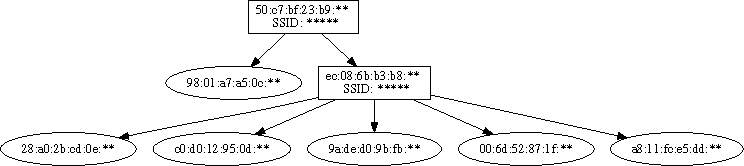
\includegraphics{images/img14censored.pdf}
	\caption{Settimo esempio}
	\label{fig:es7}
\end{figure}

\subsubsection{Reti complesse}
Sebbene la libreria per la ricostruzione della topologia Wi-Fi sia stata sviluppata per un funzionamento su reti locali domestiche sono stati effettuate anche delle prove su reti professionali di medie dimensioni.
In questo caso, poich\`e non si conosce l'effettiva topologia della rete, non si \'e in grado di determinare l'efficacia della soluzione proposta se non constatando la presenza di dispositivi personali collegati.
Queste prove hanno per\`o mostrato come la libreria sia in grado di distinguere tra diversi SSID annunciati dallo stesso dispositivo di rete, una peculiarit\`a presente in access point di fascia alta.


\begin{figure}[!h]
	\centering
	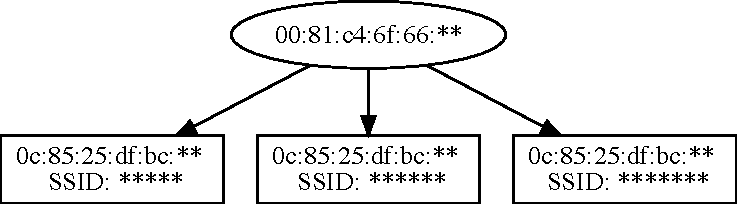
\includegraphics{images/img15censored.pdf}
	\caption{Ottavo esempio}
	\label{fig:es8}
\end{figure}

%Biblioteca

\section{Rilevazione di disservizi}




\section{Analisi delle prestazioni}
